\documentclass[conference]{IEEEtran}
\usepackage{booktabs}
\usepackage{graphicx}
\usepackage{rotating}

\title{Analyzing Open Source Plugin Ecosystems: A Mixed-Methods Approach}

\author{
\IEEEauthorblockN{Seçkin Alp Kargı}
\IEEEauthorblockA{Bilkent University\\Ankara, Türkiye\\alp.kargi@ug.bilkent.edu.tr}
\and
\IEEEauthorblockN{Anıl Koyuncu}
\IEEEauthorblockA{Bilkent University\\Ankara, Türkiye\\anil.koyuncu@cs.bilkent.edu.tr}
}

\begin{document}
\begin{abstract}
Plugin ecosystems extend host platforms with third-party functionality and are mediated by marketplaces that coordinate distribution and updates. At ecosystem scale, openness introduces complex dependency chains, governance variation, and supply-chain exposure, yet prior empirical work is typically single-platform or single-dimension and lacks unified analysis of governance, supply-chain signals, and plugin semantics. This paper presents a cross-platform empirical study of nine plugin marketplaces using a large-scale snapshot of marketplace data and a deep subset of GitHub-hosted plugins. The study combines repository mining, supply-chain security signals, and large language model (LLM)-assisted semantic classification to characterize ecosystem health, maintenance signals, and functional roles. Results show substantial heterogeneity in governance and responsiveness across platforms, uneven and incomplete supply-chain hygiene signals, concentration of engagement and maintenance effort in a small subset of plugins, and the feasibility of LLM-assisted standardization of functional descriptions. The resulting dataset and measurement pipeline provide a reusable basis for comparative analysis and offer practical relevance for platform owners, plugin maintainers, and researchers. This study answers three research questions on ecosystem health, supply-chain hygiene, and plugin functionality across diverse plugin marketplaces.
\end{abstract}
\maketitle

\section{Introduction}
Plugin ecosystems are socio-technical marketplaces where third-party developers extend a host platform through add-ons distributed via a shared marketplace. They are central to modern software: browsers, IDEs, content management systems, and domain-specific tools rely on extensions to supply specialized functionality while keeping the core product compact and stable. Marketplaces coordinate discovery, updates, and reputation signals, and they connect thousands of independent projects to large user populations. They also expose metadata such as permissions, descriptions, and ratings that users rely on to judge suitability, while the underlying code lives in external repositories. Openness is accompanied by a larger attack surface and longer dependency chains, and the update channel presents additional trust decisions at installation time and during upgrades. Plugin ecosystems involve long-lived dependency relationships between host platforms, plugins, and third-party libraries, and these relationships change as platforms evolve. Each plugin exposes platform APIs and data flows that are visible to users only through marketplace metadata and documentation. At scale, the ecosystem is more than a collection of isolated repositories: it is a coordination layer that mediates how extension code is discovered, installed, and maintained across many hosts.

At ecosystem scale, governance, maintenance, and supply-chain health are central concerns. Governance artifacts such as licenses, Codes of Conduct, CONTRIBUTING files, and security policies provide visible signals, but their presence and quality vary across ecosystems. Many plugins are maintained by small teams or a single owner, and ownership concentration can be high even in large marketplaces; the distribution of contributors often reflects a small core with many casual participants. Abandonment and maintainer turnover appear in long-tail projects, while issue trackers and pull-request backlogs vary widely in responsiveness. Dependency stacks evolve unevenly, with some plugins keeping pace with upstream releases and others accumulating outdated or unpinned packages. These signals are part of how platform operators and users interpret reliability and risk, and the allocation of review and support resources is difficult in this setting. A cross-platform view helps reveal how such conditions differ across marketplace models, update cultures, and user communities.

Prior studies typically focus on a single ecosystem and report metrics that are difficult to align across platforms, leaving fragmented evidence on governance, engagement, and supply-chain signals. Analyses often target packaging ecosystems or individual plugin markets, and they tend to emphasize either security incidents or evolution trends rather than unified, cross-platform measurement. Cross-marketplace comparisons remain limited, and many analyses treat plugins as a homogeneous category despite differences in host platform APIs, review regimes, and dependency conventions. Moreover, existing work rarely connects quantitative repository telemetry with the semantics of what plugins do. Marketplace categories, repository tags, and documentation vary in coverage and specificity, and functionality spans a wide range of roles that are not captured by metadata alone. Manual classification at this scale is costly, and platform-specific taxonomies often mix functionality with marketing labels; comparability remains limited. Functionality patterns across ecosystems remain weakly characterized and hard to compare.

This study analyzes nine plugin marketplaces: Chrome, Firefox, VS Code, JetBrains, Sublime, WordPress, Minecraft (Modrinth), Obsidian, and Home Assistant. We assemble a global snapshot of 623{,}871 plugins/extensions and identify 86{,}120 open-source plugins with public GitHub repositories, establishing the scale of openness across diverse platforms. For in-depth analysis we examine the top-100 GitHub-hosted plugins per platform (900 total), which together account for 6.1 billion downloads and 2.24 million GitHub stars; after deduplication the subset maps to 822 unique GitHub repositories. The global snapshot provides ecosystem-wide context, while the deep subset supports repository-level measurement of governance and supply-chain signals. The analysis combines repository mining with LLM-assisted semantic analysis of documentation and derives measurements of governance, maintenance, and supply-chain indicators alongside functionality signals. The top-100 focus reflects the most visible projects per platform and offers consistent sampling across ecosystems with very different sizes, with deeper inspection centered on repositories that attract high user attention.

This framing yields three research questions. RQ1 examines ecosystem health and governance, asking how contribution practices, ownership concentration, and responsiveness vary across marketplaces. RQ2 focuses on supply-chain hygiene and security signals, including dependency practices, update activity, and maintenance responsiveness in the deep subset. RQ3 characterizes plugin functionality patterns through LLM-assisted analysis of documentation and metadata, with cross-platform comparisons of what plugins do beyond platform-specific categories and uneven marketplace taxonomies.

This paper contributes a cross-platform dataset and curated snapshot, a mixed-method measurement pipeline that combines marketplace data, repository mining, and semantic analysis, empirical findings that compare governance and supply-chain signals across nine ecosystems, and implications for platform operators, plugin maintainers, and researchers. The paper is organized as follows. Section 2 discusses background on plugin ecosystems and governance concepts. Section 3 details data collection and analysis methods. Section 4 reports empirical results, and Section 5 discusses threats to validity and related work. Section 6 concludes.

\section{Background}

\subsection{Software and Plugin Ecosystems}
Software ecosystems describe communities of actors and artifacts organized around a core platform, including complementors, shared APIs, and supporting infrastructures for coordination and distribution \cite{manikas2013ecosystem,mens2014ecosystems}. Plugin ecosystems are a specific form in which extensions integrate with host platforms via published extension points, enabling functionality that is developed and maintained outside the platform core \cite{wu2021browserextensions,decan2019empirical}. Marketplaces mediate discovery, distribution, and updates, and they provide metadata and policy enforcement surfaces that shape how plugins are presented and maintained.

Cross-platform comparison is non-trivial because ecosystems differ in governance models, review pipelines, packaging conventions, and marketplace scale, and these differences influence how comparable signals are collected and interpreted across platforms \cite{decan2019empirical}. As a result, a background framing is needed to clarify how platform context shapes marketplace operations and plugin lifecycles.

\subsection{Marketplace Governance and Review Policies}
Marketplace governance is implemented through a combination of review models, source and packaging constraints, and trust signals. We distinguish three policy dimensions: (A) \emph{review model} (manual, automated, hybrid, or PR-based listing), (B) \emph{source/packaging constraint} (source-required, packaged artifact, PR-based/git-hosted, or manifest validation), and (C) \emph{primary trust signal} (human review, verified publisher, verifier report, community PR, or manifest checks). These dimensions vary across browsers, IDEs, CMS platforms, gaming, and specialized tools, which frames cross-platform comparisons of plugin practices.

\begin{table*}[t]
\centering
\small
\begin{tabular}{l p{2.6cm} p{5.0cm} p{3.0cm}}
\hline
Platform & Review Type & Source / Packaging Policy & Primary Trust Signal \\
\hline
Chrome & Automated / risk-based & Packaged extensions; remote code restricted & Policy compliance checks \\
Firefox & Manual initial, automated updates & Submitted source required for review & Human code review \\
VS Code & Automated & Marketplace package; optional source link & Verified publisher identity \\
JetBrains & Hybrid (automated + manual) & Marketplace package with verifier checks & Plugin verifier report \\
Sublime & PR-based listing & Git-hosted packages tracked by tags & Community PR merge \\
WordPress & Manual & SVN-hosted plugins; GPL-compatible & SVN history and review checks \\
Modrinth & Manual moderation & Packaged mods with metadata manifest & Moderation decision \\
Obsidian & Manual initial & Bundled JavaScript plugins & Desktop security audit \\
Home Assistant (HACS) & PR-based + automated checks & GitHub release + manifest file & Manifest validation \\
\hline
\end{tabular}
\caption{Condensed marketplace policy matrix.}
\label{tab:policy_matrix}
\end{table*}

These policy dimensions provide context for interpreting repository-level signals such as governance artifacts, workflow usage, dependency hygiene, and security tooling coverage. They may co-occur with observed platform differences, but the policy matrix is a descriptive snapshot and does not imply causal effects.

\subsection{Governance and Community Health in Open Source}
Governance artifacts such as licenses, Codes of Conduct, CONTRIBUTING guides, and security policies provide visible signals about contributor expectations and project practices \cite{li2021coc,fronchetti2023contributing}. Ownership concentration relates to bus-factor risk and resilience to maintainer turnover, providing a structural view of how responsibilities are distributed \cite{avelino2016truck}. Issue and pull-request responsiveness are commonly used as proxies for community health, capturing aspects of maintenance attention and collaboration.

Repository-based signals are informative but imperfect. GitHub data can be shaped by automation, missing metadata, and off-platform coordination, which complicates direct inference about community processes \cite{kalliamvakou2014promises}. These limitations motivate careful interpretation of governance and health indicators across ecosystems.

\subsection{Supply-Chain Risks in Plugin Ecosystems}
Plugins function as supply-chain dependencies because they bring external code and transitive libraries into host environments. Dependency footprints can be complex, and transitive relationships make risk assessment non-trivial across platforms \cite{decan2019empirical}. Stale dependencies and update lag are common concerns in software ecosystems, and measures such as LibYear characterize temporal distance between deployed and available dependencies \cite{cox2015libyear,kula2018impact}. Plugin-specific security concerns have been discussed in contexts such as WordPress and Minecraft, underscoring the diversity of risk surfaces across ecosystems \cite{murphy2021plugins,lee2020minecraft}.

SBOMs provide transparency into dependency composition and can support automated vulnerability scanning and security signaling. These mechanisms are increasingly used to describe dependency structure and to surface exposure indicators without requiring manual inspection.

\subsection{LLM-Assisted Repository Analysis}
Understanding what plugins do at scale is challenging because marketplace tags, short descriptions, and repository documentation vary in coverage and specificity. Functionality may be described with different vocabulary across platforms, and metadata often reflects platform-specific conventions rather than a consistent taxonomy. Language-model-based analyses of software artifacts have been explored for repository mining and semantic tasks \cite{hindle2012naturalness,allamanis2018survey}.

LLMs can map heterogeneous text into standardized labels, supporting cross-platform comparisons of functionality when direct metadata is inconsistent \cite{demartino2025primes,vaswani2017attention}. Responsible use emphasizes fixed label sets, conservative prompting, and confidence reporting, alongside explicit acknowledgment of hallucination and bias risks in automated semantic analysis \cite{demartino2025primes}.

\section{Research Questions}

This section formulates research questions to structure a cross-platform, multi-dimensional analysis of plugin ecosystems. The questions align with background dimensions of governance, supply-chain signals, and functionality, and are framed to support measurable, comparable analyses across heterogeneous marketplaces.

\subsection{RQ1: Ecosystem Health and Governance}
\textbf{How do scale, engagement, governance maturity, ownership concentration, and responsiveness vary across plugin ecosystems, and what relationships emerge among these signals?}
This question is operationalized by examining ecosystem scale through total plugins and open-source availability, engagement through usage and attention indicators and their concentration, governance maturity through the presence of formal governance artifacts and continuous integration workflows, ownership concentration through relative contribution shares of maintainers and core teams, and responsiveness and maintenance risk through issue handling, pull-request turnaround, and signs of abandonment.

\subsection{RQ2: Supply-Chain Hygiene and Security Signals}
\textbf{What supply-chain hygiene and security signals characterize popular plugins across ecosystems?}
This question is operationalized by analyzing dependency footprint and freshness, the availability of software bills of materials, exposure to publicly reported vulnerabilities, and automated security posture signals from widely used assessment tools.

\subsection{RQ3: Plugin Functionality and Semantic Patterns}
\textbf{What functionality patterns dominate plugin ecosystems, and how reliably can LLM-assisted analysis standardize heterogeneous marketplace descriptions?}
This question is operationalized by classifying repositories into generic and platform-specific functionality categories, assessing coverage and confidence of semantic classification, and accounting for incomplete or missing documentation.

\section{Study Design}

\begin{figure}[t]
\centering
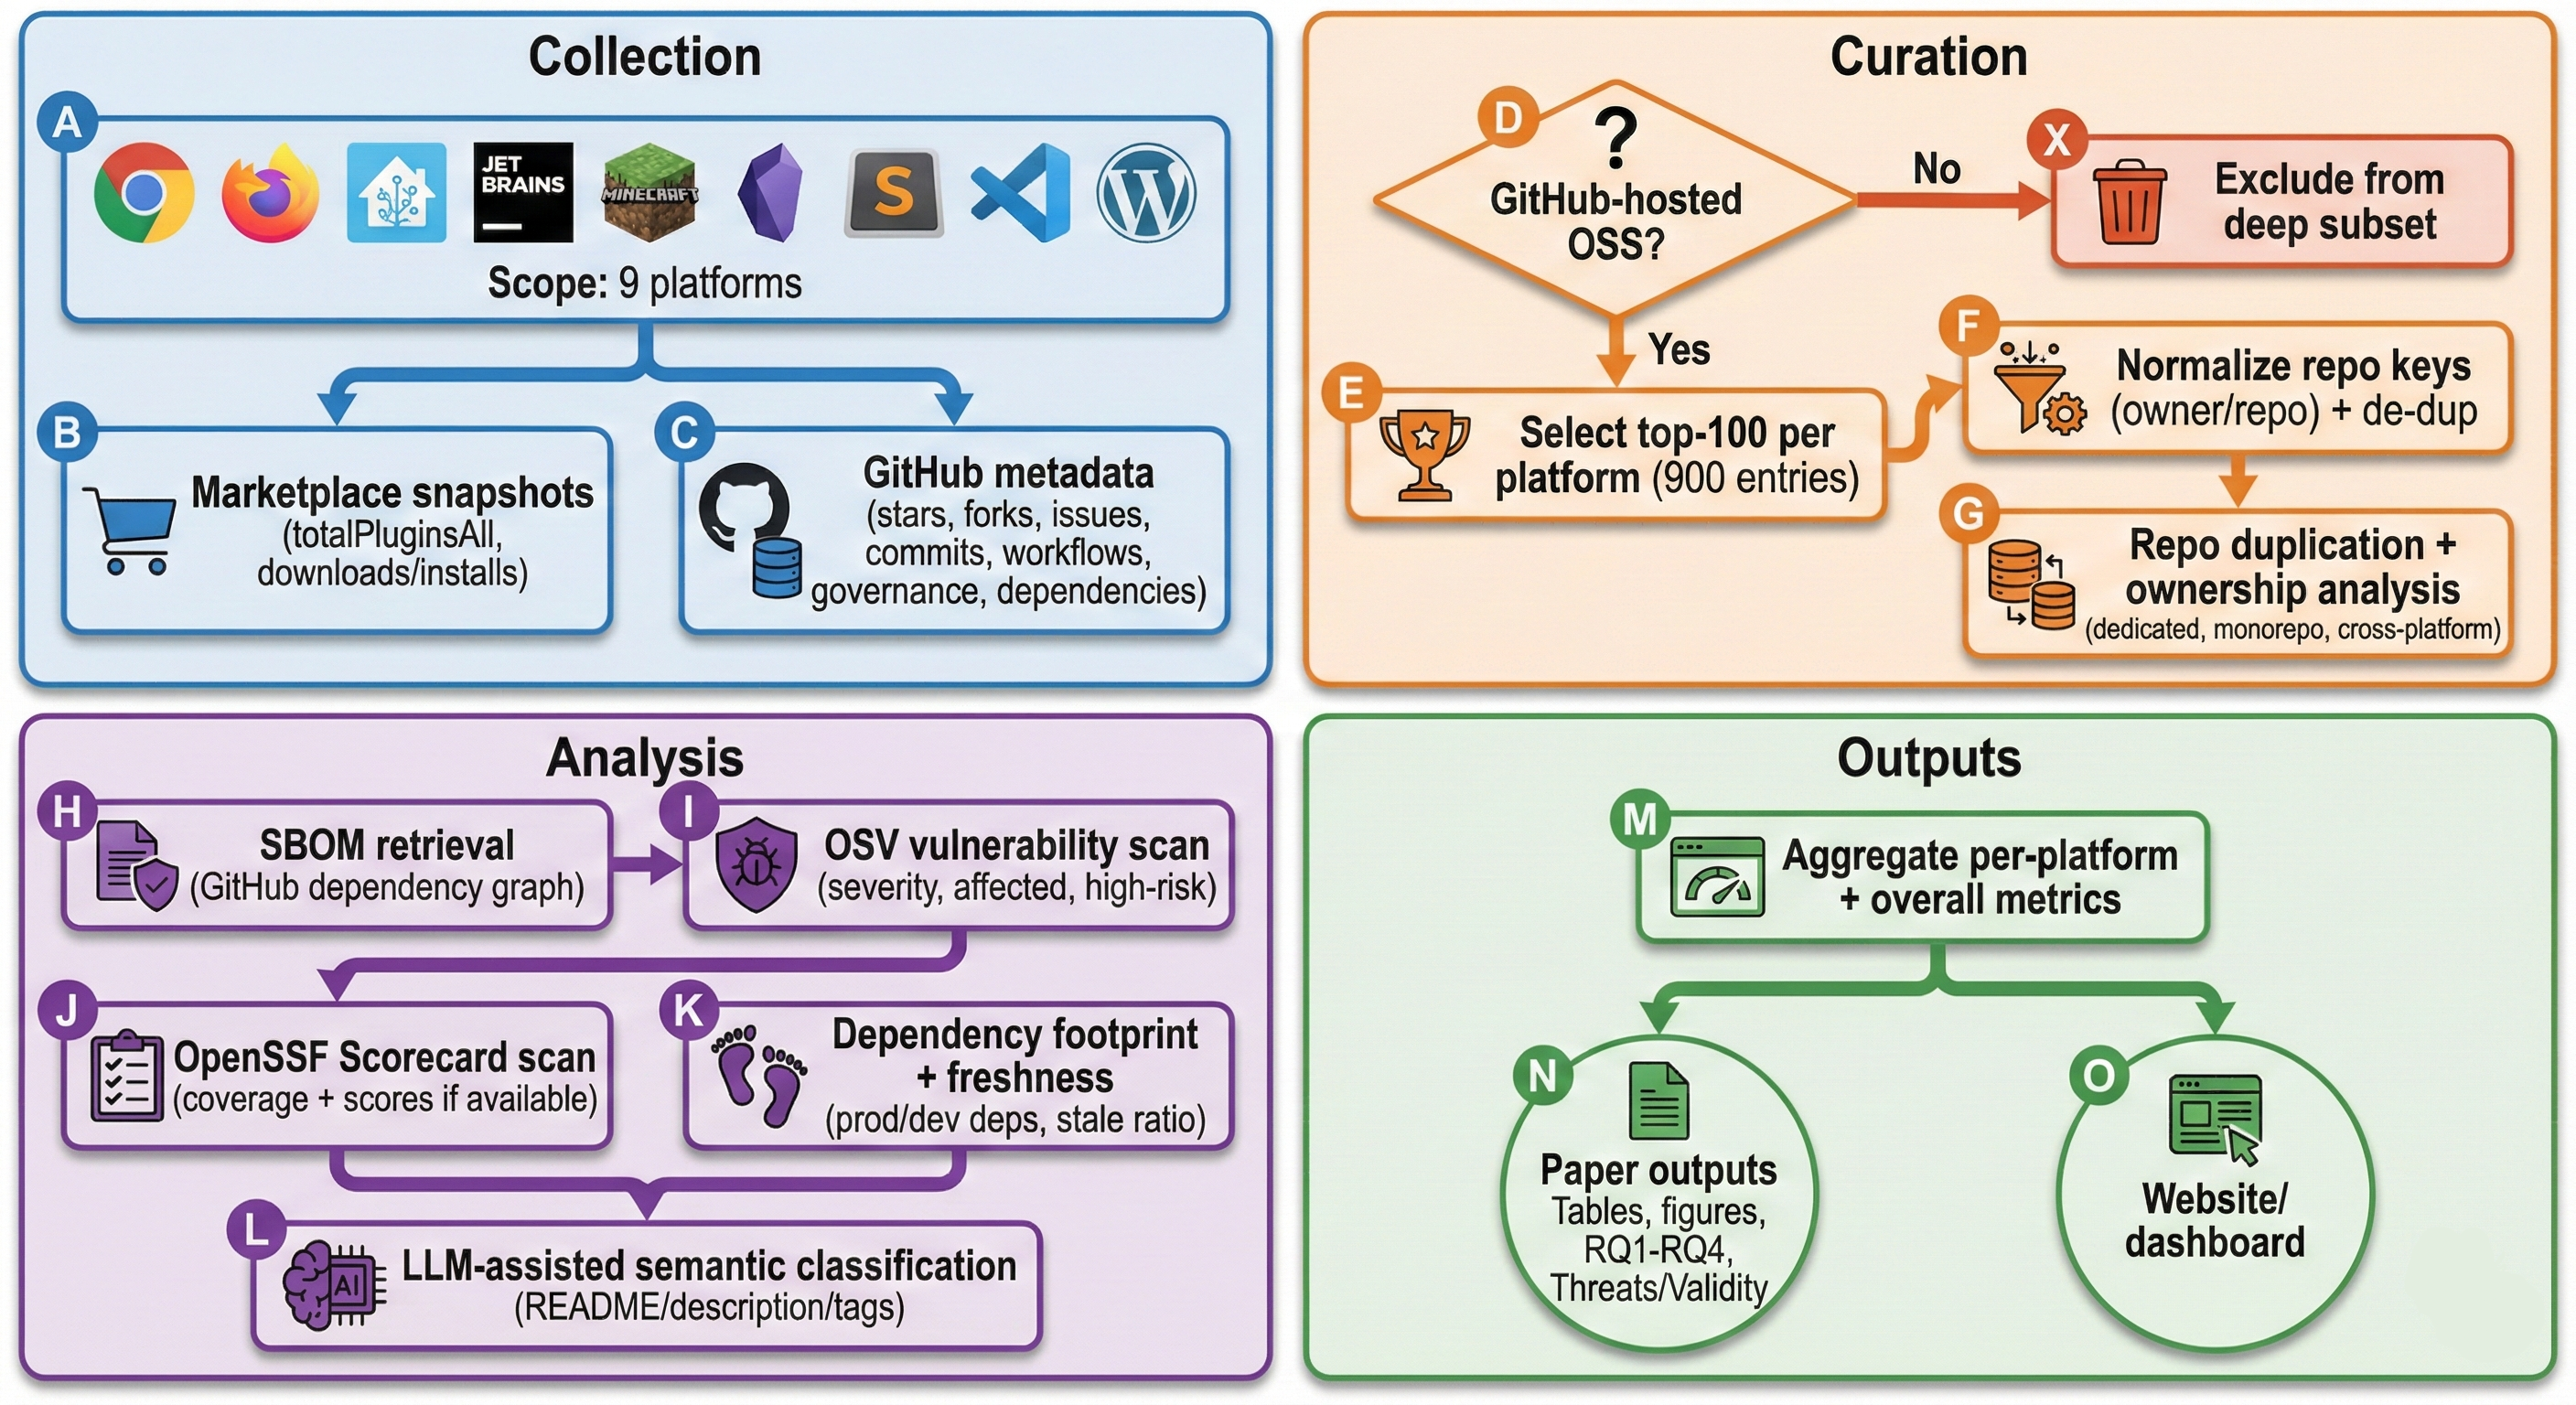
\includegraphics[width=\columnwidth]{flow.png}
\caption{Overview of the data collection and analysis pipeline.}
\label{fig:pipeline_flow}
\end{figure}

\subsection{Dataset and Sampling}
The study covers nine plugin marketplaces: Chrome, Firefox, VS Code, JetBrains, Sublime, WordPress, Minecraft (Modrinth), Obsidian, and Home Assistant. The global snapshot contains 623{,}871 plugins/extensions, of which 86{,}120 are open-source plugins with public GitHub repositories. For deep analysis, we select the top-100 GitHub-hosted plugins per platform (900 total). This fixed-size slice targets widely used and visible plugins across ecosystems and supports consistent cross-platform comparison while acknowledging that attention in marketplaces is typically concentrated in a small fraction of entries. Because multiple plugins can point to the same repository, entries are deduplicated by canonical GitHub repository identifiers, yielding 822 unique repositories. Plugin-level records remain for marketplace-scale context, and repository-level measures are computed on the deduplicated set, including cases where a single repository is shared across plugins or platforms.

\subsection{Data Collection}
Marketplace snapshots provide platform-scale counts and download or install signals from official marketplaces \cite{chrome_store_stats,firefox_addons_stats,vscode_marketplace_stats,jetbrains_marketplace_stats,wordpress_plugin_stats,modrinth_stats,obsidian_stats,homeassistant_hacs_stats,sublime_package_control_stats}. Repository metadata is gathered via the GitHub REST API, including stars, forks, issues, commits, workflows, and governance files \cite{githubapi}. Dependency manifests are extracted when available to characterize declared dependencies and update practices. External tooling is used to generate SBOMs, query public vulnerability databases, and derive automated security assessment signals from repository artifacts.

\subsection{Measures and Metrics}
\paragraph{Supply-Chain Signals Overview.} SBOMs (software bills of materials) provide a structured inventory of direct and transitive dependencies and are used here as a transparency signal rather than a security guarantee. OSV is a public vulnerability database; an affected repository has at least one matched advisory in its dependency graph, and a high-risk repository has at least one Critical or High severity entry. OpenSSF Scorecard reports automated repository security practice signals (score range 0--10) and does not imply compliance; NA indicates a check is not applicable or lacks sufficient evidence. Coverage varies by tool applicability and data availability, and results are presented descriptively. Detailed definitions appear in Section~\ref{sec:sc_signals}.

Global measures capture platform scale, open-source availability, and engagement concentration. Scale is measured by total marketplace counts, openness by the availability of public GitHub repositories, and engagement concentration by the distribution of downloads and stars across platforms.

Deep measures are computed on the top-100 subset to characterize governance, ownership, responsiveness, dependency practices, and workflow automation. Governance maturity reflects the presence of licenses, Codes of Conduct, CONTRIBUTING guides, security policies, and CI workflows \cite{li2021coc,fronchetti2023contributing}. Ownership concentration is summarized using relative contribution shares of maintainers and core teams \cite{avelino2016truck}. Responsiveness and maintenance risk are assessed through issue and pull-request activity patterns and inactivity windows, with known limitations of repository metadata \cite{kalliamvakou2014promises}. Dependency footprint and freshness are derived from declared manifests and staleness measures grounded in prior dependency freshness concepts \cite{cox2015libyear}. Workflow activity captures the presence and use of automation in repository pipelines.

\subsection{Metric Definitions and Derivation}
We distinguish global metrics computed from the full marketplace snapshot (plugin basis) from deep metrics computed on the top-100 GitHub subset (repository basis, deduplicated to unique repos where applicable). Platform summaries report means or rates over the relevant basis, and coverage is reported when required fields are unavailable.

\paragraph{Global metrics.} \textbf{Total plugins} ($N_{all}$) counts marketplace-listed entries per platform (unit: plugins; plugin basis; full snapshot coverage). \textbf{OSS availability} is $N_{oss}/N_{all}$ where $N_{oss}$ is the count of entries with a public GitHub repository (unit: proportion; plugin basis; missing when repository links are absent). \textbf{Star concentration index} is $S_{conc}=\overline{Stars}_{top100}/\log_{10}(N_{all})$, using mean stars from the top-100 slice and platform size $N_{all}$ (unit: stars per log-scaled plugin count; plugin basis for $N_{all}$ and repo basis for stars; computed when star data are available). Higher values indicate that user attention is concentrated in fewer, highly starred plugins relative to platform size. The log scaling dampens extreme differences in platform size.

\paragraph{Deep metrics.} \textbf{Governance maturity score} is the sum of four binary indicators for the presence of a license, Code of Conduct, security policy, and CONTRIBUTING file ($0$--$4$; repo basis; missing files contribute $0$). \textbf{Workflow count} is the number of CI workflows reported by GitHub (unit: count; repo basis; coverage limited by workflow metadata availability). \textbf{Abandonment rate} is the fraction of repos whose last commit is older than 365 days (unit: proportion; repo basis; threshold: 365 days; coverage requires commit timestamps). \textbf{Issue density} is $D_{issue}=N_{open}/N_{stars}$ (unit: issues per star; repo basis; undefined when stars are zero or issues are disabled and excluded). \textbf{Issue efficiency} is $E_{issue}=(N_{closed}/N_{total})\times 1/\log(1+T_{avg\_hours})$ using closure rate and average time to close (unit: dimensionless; repo basis; computed when closure data exist). \textbf{PR friction} is the median time-to-merge for pull requests from non-owners (unit: days; repo basis; coverage limited to repos with external PRs). \textbf{Owner Share (\%)} and \textbf{Core-Team Share (Top-3, \%)} are $R_{owner}=100 \times C_{owners}/C_{total}$ and $R_{core}=100 \times C_{top3}/C_{total}$, reported as percentages (0--100) of GitHub-reported contribution counts; $C_{total}$ denotes the repository's total GitHub-reported contribution count (unit: percent; repo basis; computed when contributor statistics are available). Higher values indicate stronger concentration of contribution effort among few maintainers. \textbf{Dependency footprint} is the average number of declared production and development dependencies per repo (unit: count; repo basis; coverage limited to parsable manifests). \textbf{Stale dependency ratio} is the share of declared dependencies whose version lags the latest release (LibYear age $>0$) (unit: proportion; repo basis; missing when manifests are absent). \textbf{SBOM coverage} is the fraction of top-100 plugin entries with a successfully generated SBOM (plugin basis; coverage excludes not-found, error, or rate-limited results). \textbf{OSV coverage} and \textbf{Scorecard coverage} are the fractions of unique GitHub repositories with successful analysis (repo basis; plugin-level coverage is reported separately when needed).

\subsection{LLM-Assisted Semantic Analysis}
Plugin functionality is inferred from repository documentation and metadata, including README files, short descriptions, topics, and marketplace fields. The analysis maps inputs to fixed label sets with both generic and platform-specific categories and records confidence estimates for each classification. When documentation is missing, classification uses the remaining metadata and records missingness for coverage tracking. To avoid double counting, semantic labels are aggregated at the repository level for shared repositories.

\subsection{Analysis Plan}
Measurements are summarized per platform and compared across ecosystems using comparable scales and definitions. Relationships among engagement, governance, and supply-chain signals are examined through correlation analysis. The analysis also identifies subsets exhibiting elevated risk indicators, such as concentrated ownership or vulnerable dependency profiles, to contextualize cross-platform differences without imposing platform-specific thresholds.

\subsection{Data Availability and Research Artifacts}
The dataset used in this study is publicly available. A publicly accessible companion website supports interactive inspection of the analyzed plugins, enables downloading the complete dataset and filtered subsets, and mirrors the static snapshot used in this paper \cite{osspluginhub2025}. The website does not influence any reported results and serves only to disseminate the released data. All analyses reported in this paper are derived from the dataset described above.

\subsection{Supply-Chain Security Signals: SBOM, OSV, and Scorecard}\label{sec:sc_signals}
This study uses three complementary signals to describe supply-chain security in plugin ecosystems: SBOM availability, OSV vulnerability matching, and OpenSSF Scorecard checks. They provide observable, repository-level signals that support comparative analysis without implying compliance or security guarantees. The associated results are reported in Table~\ref{tab:rq3_osv_summary} (SBOM and OSV) and Table~\ref{tab:rq3_scorecard_full} (Scorecard).

\paragraph{SBOM.} A software bill of materials (SBOM) is a structured inventory of direct and transitive dependencies for a software artifact. It improves supply-chain transparency and enables automated vulnerability scanning by making dependency composition explicit. In this study, SBOM availability reflects tool-generated SBOMs derived from repository artifacts, not platform-mandated disclosures. SBOM coverage is defined as the share of top-100 plugin entries for which SBOM generation succeeds; not-found, error, or rate-limited outcomes are treated as missing coverage. SBOM presence indicates observability of dependencies, not security or correctness.

\paragraph{OSV.} The Open Source Vulnerabilities (OSV) database aggregates advisories from multiple ecosystems and links them to specific package versions, enabling dependency graph matching. Severity levels are reported as critical, high, medium, or low to describe advisory severity categories. In this study, an affected repository is one with at least one OSV match in its resolved dependencies; a high-risk repository has at least one critical or high severity OSV entry. Vulnerability counts summarize the number of matched advisories per repository or platform. OSV results depend on dependency resolution and database coverage and do not imply exploitability in the plugin context.

\paragraph{OpenSSF Scorecard.} OpenSSF Scorecard is an automated, repository-level assessment of security practice signals rather than vulnerabilities. Checks are grouped into code hygiene (e.g., Binary-Artifacts, License), development process (e.g., CI-Tests, Branch-Protection), dependency practices (e.g., Dependency-Update, Pinned-Dependencies), and security hardening (e.g., Security-Policy, SAST, Fuzzing, Signed-Releases). Many checks are conditional on repository characteristics and may be marked NA; low averages or high NA rates indicate limited applicability or missing evidence rather than noncompliance.

\paragraph{Scope and interpretation.} SBOM coverage is reported on a plugin basis, while OSV and Scorecard results are reported on a repository basis with unique-repo deduplication, and plugin-level coverage is reported where relevant. These signals are partial and complementary, and the results are presented as descriptive, cross-platform comparisons rather than judgments of compliance or security posture. A brief glossary appears in Section~\ref{sec:rq2_glossary} to aid interpretation of Tables~\ref{tab:rq3_osv_summary}--\ref{tab:rq3_scorecard_full}.

\section{Results}

\subsection{RQ1: Ecosystem Health and Governance}

\subsubsection{Marketplace Policy Groups and Observed Differences}
Based on the policy matrix (Table~\ref{tab:policy_matrix}), platforms can be grouped by review model:
\begin{itemize}
    \item Manual-initial/human review: Firefox, WordPress, Obsidian, Modrinth (Minecraft).
    \item Automated/risk-based: Chrome, VS Code.
    \item Hybrid: JetBrains.
    \item PR-based listing: Sublime, Home Assistant (HACS).
\end{itemize}
These groupings are used to organize descriptive comparisons; associations are correlational and may reflect other ecosystem factors.

Review models and packaging constraints shape what artifacts are submitted or reviewed, influencing observability and incentives for governance artifacts, workflow adoption, and supply-chain tooling coverage. The patterns below are correlational rather than causal, but policy context provides a lens for understanding cross-platform variation in governance artifacts, workflow adoption, and SBOM/OSV/Scorecard coverage.

Governance maturity scores and workflow counts vary within and across policy groups. The automated/risk-based group includes VS Code with governance maturity 1.73 and workflows 3.31, while Chrome reports 1.08 and 2.49. Manual-initial platforms span values such as Firefox (1.06, 1.08), WordPress (0.93, 2.59), Obsidian (0.81, 1.13), and Modrinth/Minecraft (0.80, 1.24). PR-based listing shows low values for Sublime (0.46, 0.21) alongside higher workflow usage for Home Assistant (0.95, 3.18) (Table~\ref{tab:rq2_governance}).

Responsiveness and maintenance signals also vary across groups. Issue efficiency ranges from 0.467 (JetBrains) to 0.707 (Home Assistant), while abandonment spans 0.03 (Modrinth/Minecraft) to 0.79 (Sublime). Issue density is lowest in JetBrains (0.01837) and highest in WordPress (0.35500), indicating heterogeneous maintenance loads within each review model category (Tables~\ref{tab:rq1_scale} and~\ref{tab:rq2_governance}).

Dependency freshness does not align uniformly with policy groupings. Stale dependency ratios are high in Obsidian (0.78) and VS Code (0.66), moderate in Chrome (0.59) and WordPress (0.63), and low in JetBrains (0.15), Sublime (0.07), and Modrinth/Minecraft (0.06) (Table~\ref{tab:rq2_deps}).

Supply-chain tooling coverage varies across platforms irrespective of review model. SBOM coverage ranges from 98.0\% (VS Code) to 63.0\% (Modrinth/Minecraft), OSV coverage from 86.7\% (VS Code) to 54.0\% (Modrinth/Minecraft), and Scorecard mean scores from 4.37 (VS Code) to 2.78 (Obsidian) and 2.81 (Sublime) (Tables~\ref{tab:rq3_osv_summary} and~\ref{tab:rq3_scorecard_full}). These differences co-occur with platform governance and dependency signals but are descriptive and not interpreted as causal.

\paragraph{Findings.} (F1) Governance maturity and workflow usage co-occur with policy categories but show substantial within-group spread, from VS Code (1.73, 3.31) and Chrome (1.08, 2.49) to Sublime (0.46, 0.21) and Home Assistant (0.95, 3.18) (Table~\ref{tab:rq2_governance}). (F2) Responsiveness signals vary widely across groups, with issue efficiency spanning 0.467 (JetBrains) to 0.707 (Home Assistant) and abandonment ranging from 0.03 (Modrinth/Minecraft) to 0.79 (Sublime) (Tables~\ref{tab:rq1_scale} and~\ref{tab:rq2_governance}). (F3) Dependency staleness differs across platforms, from Obsidian at 0.78 and VS Code at 0.66 to Modrinth/Minecraft at 0.06 and Sublime at 0.07 (Table~\ref{tab:rq2_deps}). (F4) Supply-chain tooling coverage and Scorecard means vary, with SBOM coverage 98.0\% (VS Code) versus 63.0\% (Modrinth/Minecraft), OSV coverage 86.7\% (VS Code) versus 54.0\% (Modrinth/Minecraft), and Scorecard means 4.37 (VS Code) versus 2.81 (Sublime) (Tables~\ref{tab:rq3_osv_summary} and~\ref{tab:rq3_scorecard_full}).

\subsubsection{Scale and Engagement}
Platform scale varies by orders of magnitude. Total marketplace counts range from 2{,}656 plugins in Obsidian to 246{,}379 in Chrome, and open-source plugins with public GitHub repositories range from 2{,}389 in Home Assistant to 26{,}089 in Minecraft (Table~\ref{tab:platform_overview}). Top-100 totals also vary substantially: stars span 30{,}385 (Minecraft) to 791{,}751 (Chrome), downloads span 4{,}356{,}695 (Home Assistant) to 2{,}950{,}813{,}730 (VS Code), issues span 1{,}786 (Sublime) to 33{,}724 (Chrome), and forks span 7{,}912 (Sublime) to 138{,}394 (JetBrains) (Table~\ref{tab:platform_overview}).

\begin{table*}[t]
\caption{Platform-scale overview (top-100 GitHub subset per platform).}
\label{tab:platform_overview}
\resizebox{\textwidth}{!}{%
\begin{tabular}{lcccccccc}
\toprule
\textbf{Platform} & \textbf{Category} & \textbf{All Plugins} & \textbf{OSS GitHub} & \textbf{Top-100 Size} & \textbf{Stars (Top-100)} & \textbf{Downloads (Top-100)} & \textbf{Issues (Top-100)} & \textbf{Forks (Top-100)} \\
\midrule
Chrome & Browser & 246{,}379 & 7{,}459 & 100 & 791{,}751 & 233{,}670{,}000 & 33{,}724 & 120{,}128 \\
Firefox & Browser & 110{,}320 & 7{,}862 & 100 & 479{,}809 & 17{,}242{,}577 & 12{,}156 & 81{,}394 \\
JetBrains & IDE & 10{,}003 & 5{,}849 & 100 & 501{,}545 & 587{,}304{,}466 & 9{,}213 & 138{,}394 \\
VS Code & IDE & 86{,}145 & 25{,}136 & 100 & 184{,}466 & 2{,}950{,}813{,}730 & 32{,}550 & 35{,}166 \\
Sublime & IDE & 5{,}581 & 4{,}694 & 100 & 59{,}452 & 49{,}475{,}544 & 1{,}786 & 7{,}912 \\
WordPress & CMS & 59{,}000 & 3{,}986 & 100 & 31{,}718 & 7{,}180{,}000 & 11{,}260 & 9{,}336 \\
Minecraft & Gaming & 98{,}600 & 26{,}089 & 100 & 30{,}385 & 2{,}217{,}620{,}403 & 5{,}332 & 6{,}984 \\
Obsidian & Specialized & 2{,}656 & 2{,}656 & 100 & 91{,}575 & 38{,}734{,}337 & 8{,}972 & 6{,}932 \\
Home Assistant & Specialized & 5{,}187 & 2{,}389 & 100 & 71{,}025 & 4{,}356{,}695 & 5{,}513 & 8{,}487 \\
\midrule
\textbf{Total} & --- & 623{,}871 & 86{,}120 & 900 & 2{,}241{,}726 & 6{,}106{,}397{,}752 & 120{,}506 & 414{,}733 \\
\bottomrule
\end{tabular}%
}
\end{table*}

Average engagement within the top-100 subset spans wide ranges (Table~\ref{tab:rq1_scale}). Average stars range from 303.85 (Minecraft) to 7{,}917.51 (Chrome), and average downloads range from 43{,}566.95 (Home Assistant) to 29{,}508{,}137.30 (VS Code). The star concentration index ranges from 68.80 (Minecraft) to 3{,}287.67 (Chrome), with intermediate values such as 1{,}331.39 (JetBrains) and 419.21 (VS Code), indicating substantial variation in attention concentration across ecosystems.

\begin{table}[t]
\caption{Platform scale and engagement (top-100 GitHub subset; higher star concentration indicates attention concentrated in few highly starred plugins).}
\label{tab:rq1_scale}
\resizebox{\columnwidth}{!}{%
\begin{tabular}{lrrrrrrrr}
\toprule
\textbf{Platform} & \textbf{All} & \textbf{OSS} & \textbf{Avg Stars} & \textbf{Avg Downloads} & \textbf{Issue Density} & \textbf{Abandon.} & \textbf{Star Conc. Idx} \\
\midrule
Chrome & 246{,}379 & 7{,}459 & 7{,}917.51 & 2{,}336{,}700.00 & 0.04259 & 0.26 & 3{,}287.67 \\
Firefox & 110{,}320 & 7{,}862 & 4{,}798.09 & 172{,}425.77 & 0.02534 & 0.43 & 1{,}231.69 \\
JetBrains & 10{,}003 & 5{,}849 & 5{,}015.45 & 5{,}873{,}044.66 & 0.01837 & 0.18 & 1{,}331.39 \\
VS Code & 86{,}145 & 25{,}136 & 1{,}844.66 & 29{,}508{,}137.30 & 0.17646 & 0.24 & 419.21 \\
Sublime & 5{,}581 & 4{,}694 & 594.52 & 494{,}755.44 & 0.03004 & 0.79 & 161.93 \\
WordPress & 59{,}000 & 3{,}986 & 317.18 & 71{,}800.00 & 0.35500 & 0.34 & 88.09 \\
Minecraft & 98{,}600 & 26{,}089 & 303.85 & 22{,}176{,}204.03 & 0.17548 & 0.03 & 68.80 \\
Obsidian & 2{,}656 & 2{,}656 & 915.75 & 387{,}343.37 & 0.09797 & 0.47 & 267.43 \\
Home Assistant & 5{,}187 & 2{,}389 & 710.25 & 43{,}566.95 & 0.07762 & 0.34 & 210.24 \\
\bottomrule
\end{tabular}%
}
\end{table}

\subsubsection{Governance Maturity and Ownership}
Governance maturity varies by platform, with governance maturity scores spanning 0.46 (Sublime) to 1.73 (VS Code) and a reported cross-platform average of 1.009/4 (Table~\ref{tab:rq2_governance}). Workflow counts range from 0.21 (Sublime) to 3.31 (VS Code). Ownership concentration also varies: Core-Team Share (Top-3, \%) ranges from 0.000 (Sublime, Home Assistant) to 31.302 (VS Code), and Owner Share (\%) ranges from 5.93 (Sublime) to 40.46 (Minecraft) (Table~\ref{tab:rq2_governance}).

\begin{table}[t]
\caption{Governance and ownership metrics (top-100 GitHub subset; shares are reported as percentages of total GitHub-reported contributions).}
\label{tab:rq2_governance}
\resizebox{\columnwidth}{!}{%
\begin{tabular}{lrrrrr}
\toprule
\textbf{Platform} & \textbf{Gov. Score} & \textbf{Workflows} & \textbf{Core-Team Share (Top-3, \%)} & \textbf{Owner Share (\%)} & \textbf{Issue Eff.} \\
\midrule
Chrome & 1.08 & 2.49 & 6.247 & 17.99 & 0.696 \\
Firefox & 1.06 & 1.08 & 0.799 & 31.57 & 0.628 \\
JetBrains & 1.26 & 2.71 & 1.223 & 14.03 & 0.467 \\
VS Code & 1.73 & 3.31 & 31.302 & 7.44 & 0.509 \\
Sublime & 0.46 & 0.21 & 0.000 & 5.93 & 0.675 \\
WordPress & 0.93 & 2.59 & 0.272 & 28.29 & 0.658 \\
Minecraft & 0.80 & 1.24 & 1.899 & 40.46 & 0.657 \\
Obsidian & 0.81 & 1.13 & 6.143 & 31.37 & 0.523 \\
Home Assistant & 0.95 & 3.18 & 0.000 & 30.78 & 0.707 \\
\bottomrule
\end{tabular}%
}
\end{table}

Ownership mix is dominated by community plugins (765/900, 85.0\%), with official plugins at 119/900 (13.2\%) and corporate plugins at 16/900 (1.8\%). Platform standouts include JetBrains (45/100 official) and VS Code (40/100 official), while Home Assistant and Minecraft are entirely community (100/100 each). Shared official repositories include JetBrains/intellij-community (19 plugins) and Microsoft/vscode-remote-release (6 plugins), indicating multiple plugins per repository within the top-100 subset.

Language and license distributions contextualize governance artifacts in the top-100 set (Table~\ref{tab:rq2_dist}). TypeScript (258, 28.7\%), JavaScript (186, 20.7\%), and Java (152, 16.9\%) dominate, followed by Python (89, 9.9\%) and PHP (89, 9.9\%). Licensing is led by MIT (341, 37.9\%) and No License (145, 16.1\%), followed by Other (98, 10.9\%) and GPLv3 (90, 10.0\%), with Apache 2.0 at 72 (8.0\%).

\begin{table}[t]
\caption{Top languages and licenses across the 900-plugin top subset.}
\label{tab:rq2_dist}
\resizebox{\columnwidth}{!} & \textbf{License} & \textbf{Count} & \textbf{\%} \\
\midrule
TypeScript & 258 & 28.7 & MIT & 341 & 37.9 \\
JavaScript & 186 & 20.7 & No License & 145 & 16.1 \\
Java & 152 & 16.9 & Other & 98 & 10.9 \\
Python & 89 & 9.9 & GPLv3 & 90 & 10.0 \\
PHP & 89 & 9.9 & Apache 2.0 & 72 & 8.0 \\
Unknown & 51 & 5.7 & GPLv2 & 45 & 5.0 \\
Kotlin & 34 & 3.8 & MPL 2.0 & 30 & 3.3 \\
CSS & 7 & 0.8 & LGPL v3 & 27 & 3.0 \\
Dockerfile & 6 & 0.7 & AGPL v3 & 13 & 1.4 \\
HTML & 5 & 0.6 & BSD-3-Clause & 12 & 1.3 \\
\bottomrule
\end{tabular}%
}
\end{table}

\subsubsection{Responsiveness and Maintenance Risk}
Responsiveness measures vary across platforms (Tables~\ref{tab:rq1_scale} and~\ref{tab:rq2_governance}). Issue density ranges from 0.01837 (JetBrains) to 0.35500 (WordPress). Issue efficiency ranges from 0.467 (JetBrains) to 0.707 (Home Assistant). Abandonment ranges from 0.03 (Minecraft) to 0.79 (Sublime), with intermediate values such as 0.47 (Obsidian) and 0.34 (WordPress and Home Assistant). PR friction (median time-to-merge for external contributors) is reported at around 22 days in the top-100 subset.

\subsubsection{Relationships Among Ecosystem Signals}
At the aggregate level, governance maturity is reported alongside issue efficiency of 0.613 and abandonment of 12.8\%, and these associations are described as correlational. At platform level, governance scores and issue efficiency do not follow a single ordering: VS Code pairs a governance score of 1.73 with issue efficiency 0.509, Chrome pairs 1.08 with 0.696, and JetBrains pairs 1.26 with 0.467 (Table~\ref{tab:rq2_governance}). Workflow usage and issue efficiency similarly show mixed co-occurrence, with Home Assistant (3.18 workflows, 0.707 issue efficiency), VS Code (3.31, 0.509), and Sublime (0.21, 0.675) spanning the range in Table~\ref{tab:rq2_governance}. Ownership concentration and abandonment also vary without a monotonic pattern: Minecraft combines high Owner Share (40.46\%) with low abandonment (0.03), Firefox combines high Owner Share (31.57\%) with higher abandonment (0.43), and Sublime combines low Owner Share (5.93\%) with the highest abandonment (0.79) (Tables~\ref{tab:rq2_governance} and~\ref{tab:rq1_scale}). These relationships are descriptive and correlational. Governance maturity does not correlate cleanly with responsiveness indicators, which is expected in socio-technical ecosystems where maintainer capacity, community norms, and platform context vary.

Do platform policies appear to shape observable ecosystem behavior? The evidence is mixed: automated review platforms such as VS Code co-occur with higher governance maturity, workflow adoption, and tooling coverage, while PR-based ecosystems diverge, with Sublime showing low governance and workflow signals and Home Assistant showing higher workflow use (Tables~\ref{tab:rq2_governance} and~\ref{tab:rq3_scorecard_full}). Manual-review platforms do not form a uniform cluster, spanning from low abandonment in Modrinth/Minecraft to higher abandonment in Firefox and Obsidian (Table~\ref{tab:rq1_scale}). These patterns are descriptive and consistent with policy context influencing observability and incentives, without supporting causal claims.

\subsection{RQ2: Supply-Chain Hygiene and Security Signals}

\paragraph{Supply-Chain Security Signals (Overview).}\label{sec:rq2_glossary} SBOMs provide a structured inventory of direct and transitive dependencies and are used here as a transparency signal rather than a security guarantee. In this paper, SBOM coverage denotes successful SBOM generation for a top-100 entry. OSV is a public vulnerability database that matches advisories to dependency versions; affected repositories have at least one match, and severity follows Critical/High/Medium/Low categories that indicate advisory severity rather than exploitability. OpenSSF Scorecard reports automated repository security practice signals (score range 0--10) and does not provide security guarantees; checks may be NA when not applicable or when signals are missing. Detailed definitions appear in Section~\ref{sec:sc_signals}.

\subsubsection{Dependency Footprint and Freshness}
Dependency footprints and freshness indicators vary across platforms (Table~\ref{tab:rq2_deps}). Average production dependencies range from 0.27 (Sublime) to 11.77 (Chrome), and average development dependencies range from 0.09 (Minecraft) to 19.26 (VS Code). The stale dependency ratio ranges from 0.06 (Minecraft) to 0.78 (Obsidian), with intermediate values such as 0.59 (Chrome) and 0.66 (VS Code).

\begin{table}[t]
\caption{Dependency footprint and freshness (top-100 GitHub subset).}
\label{tab:rq2_deps}
\resizebox{\columnwidth}{!}{%
\begin{tabular}{lrrr}
\toprule
\textbf{Platform} & \textbf{Avg Prod Deps} & \textbf{Avg Dev Deps} & \textbf{Stale Dep Ratio} \\
\midrule
Chrome & 11.77 & 18.86 & 0.59 \\
Firefox & 2.99 & 9.25 & 0.45 \\
JetBrains & 2.25 & 1.21 & 0.15 \\
VS Code & 6.27 & 19.26 & 0.66 \\
Sublime & 0.27 & 0.45 & 0.07 \\
WordPress & 0.96 & 8.88 & 0.63 \\
Minecraft & 3.16 & 0.09 & 0.06 \\
Obsidian & 6.06 & 19.06 & 0.78 \\
Home Assistant & 4.44 & 12.74 & 0.63 \\
\bottomrule
\end{tabular}%
}
\end{table}

\subsubsection{SBOM Availability}
SBOMs are available for 733 of 900 entries (81.4\%), with 160 not found, 3 errors, and 4 rate-limited results. Per-platform SBOM coverage ranges from 63.0\% (Minecraft) to 98.0\% (VS Code), with Chrome, JetBrains, and Obsidian at 88.0\% and Home Assistant at 87.0\% (Table~\ref{tab:rq3_osv_summary}).

\subsubsection{Vulnerability Exposure (OSV or Equivalent)}
OSV analysis covers 582 of 822 unique repositories (70.8\%) and 619 of 900 entries (68.8\%). A total of 6{,}277 vulnerabilities are reported, with 2 critical, 55 high, 537 medium, and 5{,}683 low severity findings (Table~\ref{tab:rq3_osv_summary}). Affected repositories number 285, with 297 clean repositories (49.0\% affected), and 22 repositories are classified as high-risk (3.8\%). Stale packages number 6{,}181 and old fixes 4{,}265, with 1{,}065 recent vulnerabilities; average counts are 10.79 vulnerabilities per repository and 22.02 per affected repository. Platform-level totals are highest in Chrome (1{,}476), WordPress (1{,}094), and VS Code (1{,}043). Affected rates range from 5.6\% (Minecraft) to 78.2\% (Obsidian), and high-risk rates range from 0.0\% (JetBrains, Minecraft) to 9.7\% (WordPress).

\subsubsection{Automated Security Posture Signals}
Scorecard analysis covers 645 of 819 unique repositories (78.8\%) and 675 of 900 entries (75.0\%). The mean score is 3.24 (median 2.9; p25 2.6; p75 3.7), and 74.7\% of entries fall in the 2--4 score range (Table~\ref{tab:rq3_scorecard_full}). Check-level means include Binary-Artifacts 9.67, License 8.24, and Vulnerabilities 7.33, while Branch-Protection 0.48, Security-Policy 0.76, SAST 0.40, Fuzzing 0.01, and CII-Best-Practices 0.01 are reported. CI-Tests averages 1.97 with 77.3\% coverage; Pinned-Dependencies averages 0.66 with 46.7\% coverage; Token-Permissions averages 1.06 with 45.2\% coverage; Dangerous-Workflow averages 9.87 with 45.2\% coverage; Signed-Releases averages 0.07 with 50.5\% coverage; Packaging averages 10.00 and applies to 4.6\% of repositories. NA prevalence is 55.0\% for Token-Permissions and Dangerous-Workflow and 95.2\% for Packaging.

\begin{sidewaystable*}[p]
\centering
\caption{SBOM coverage (top-100 entries) and OSV vulnerability severity by platform (unique-repo basis for OSV coverage and rates).}
\label{tab:rq3_osv_summary}
\resizebox{\textwidth}{!}{%
\begin{tabular}{lrrrrrrrrrrrr}
\toprule
\textbf{Platform} & \textbf{SBOM Cov. (\%)} & \textbf{OSV Analyzed} & \textbf{OSV Cov. (\%)} & \textbf{Affected Repos} & \textbf{Affected (\%)} & \textbf{High-Risk Repos} & \textbf{High-Risk (\%)} & \textbf{Total Vulns} & \textbf{Critical} & \textbf{High} & \textbf{Medium} & \textbf{Low} \\
\midrule
Chrome & 88.0 & 74 & 77.9 & 45 & 60.8 & 5 & 6.8 & 1{,}476 & 1 & 21 & 143 & 1{,}311 \\
Firefox & 75.0 & 68 & 68.7 & 32 & 47.1 & 2 & 2.9 & 1{,}019 & 0 & 3 & 86 & 930 \\
JetBrains & 88.0 & 48 & 71.6 & 7 & 14.6 & 0 & 0.0 & 101 & 0 & 0 & 2 & 99 \\
VS Code & 98.0 & 78 & 86.7 & 59 & 75.6 & 5 & 6.4 & 1{,}043 & 0 & 7 & 74 & 962 \\
Sublime & 68.0 & 60 & 60.0 & 4 & 6.7 & 2 & 3.3 & 155 & 0 & 8 & 3 & 144 \\
WordPress & 78.0 & 62 & 68.1 & 36 & 58.1 & 6 & 9.7 & 1{,}094 & 0 & 15 & 127 & 952 \\
Minecraft & 63.0 & 54 & 54.0 & 3 & 5.6 & 0 & 0.0 & 157 & 0 & 0 & 25 & 132 \\
Obsidian & 88.0 & 78 & 78.0 & 61 & 78.2 & 1 & 1.3 & 708 & 0 & 1 & 66 & 641 \\
Home Assistant & 87.0 & 74 & 74.0 & 49 & 66.2 & 1 & 1.4 & 811 & 1 & 0 & 43 & 767 \\
\midrule
\textbf{Overall} & 81.4 & 582 & 70.8 & 285 & 49.0 & 22 & 3.8 & 6{,}277 & 2 & 55 & 537 & 5{,}683 \\
\bottomrule
\end{tabular}%
}
\vspace{0.5cm}
\vfill
\caption{Scorecard coverage, mean scores, and check-level results by platform (top-100 entries). Cells show mean score with coverage rate (non-NA) in parentheses.}
\label{tab:rq3_scorecard_full}
\resizebox{\textwidth}{!}{%
\begin{tabular}{lrrr*{18}{r}}
\toprule
\textbf{Platform} & \textbf{Analyzed} & \textbf{Coverage (\%)} & \textbf{Mean} & \textbf{Bin-Art} & \textbf{Branch} & \textbf{CI} & \textbf{CII} & \textbf{Review} & \textbf{Contrib} & \textbf{Danger} & \textbf{Dep-Update} & \textbf{Fuzz} & \textbf{License} & \textbf{Maint} & \textbf{Pack} & \textbf{Pinned} & \textbf{SAST} & \textbf{Sec-Pol} & \textbf{Signed} & \textbf{Token} & \textbf{Vulns} \\
\midrule
Chrome & 80 & 80.0 & 3.48 & 9.85 (100.0\%) & 0.46 (100.0\%) & 3.24 (62.5\%) & 0.03 (100.0\%) & 1.36 (100.0\%) & 5.47 (100.0\%) & 9.35 (38.7\%) & 3.12 (100.0\%) & 0.00 (100.0\%) & 8.97 (100.0\%) & 4.97 (100.0\%) & 10.00 (1.2\%) & 1.56 (40.0\%) & 0.56 (100.0\%) & 1.11 (100.0\%) & 0.19 (53.8\%) & 2.45 (38.7\%) & 6.35 (100.0\%) \\
Firefox & 85 & 85.0 & 3.08 & 9.84 (100.0\%) & 0.41 (100.0\%) & 1.54 (71.8\%) & 0.05 (100.0\%) & 1.06 (100.0\%) & 4.08 (100.0\%) & 10.00 (29.4\%) & 1.53 (100.0\%) & 0.00 (100.0\%) & 8.64 (100.0\%) & 2.64 (100.0\%) & 10.00 (1.2\%) & 1.00 (30.6\%) & 0.35 (100.0\%) & 0.80 (100.0\%) & 0.00 (41.2\%) & 3.28 (29.4\%) & 7.40 (100.0\%) \\
JetBrains & 44 & 44.0 & 3.51 & 8.77 (100.0\%) & 0.66 (100.0\%) & 2.55 (65.9\%) & 0.00 (100.0\%) & 1.25 (100.0\%) & 6.48 (100.0\%) & 10.00 (45.5\%) & 1.59 (100.0\%) & 0.00 (100.0\%) & 9.48 (100.0\%) & 4.23 (100.0\%) & 10.00 (11.4\%) & 0.76 (47.7\%) & 0.84 (100.0\%) & 1.59 (100.0\%) & 0.00 (43.2\%) & 0.50 (45.5\%) & 9.16 (100.0\%) \\
VS Code & 60 & 60.0 & 4.37 & 9.88 (100.0\%) & 2.85 (100.0\%) & 3.17 (96.7\%) & 0.00 (100.0\%) & 4.30 (93.3\%) & 7.58 (100.0\%) & 10.00 (70.0\%) & 6.17 (100.0\%) & 0.00 (100.0\%) & 9.60 (100.0\%) & 3.87 (100.0\%) & -- (0.0\%) & 0.95 (71.7\%) & 1.60 (100.0\%) & 4.50 (100.0\%) & 0.00 (53.3\%) & 1.07 (70.0\%) & 4.95 (100.0\%) \\
Sublime & 92 & 92.0 & 2.81 & 9.96 (100.0\%) & 0.03 (100.0\%) & 0.65 (88.0\%) & 0.00 (100.0\%) & 1.86 (100.0\%) & 5.59 (100.0\%) & 10.00 (5.4\%) & 0.22 (100.0\%) & 0.00 (100.0\%) & 6.15 (100.0\%) & 0.25 (100.0\%) & -- (0.0\%) & 0.00 (6.5\%) & 0.00 (100.0\%) & 0.00 (100.0\%) & 0.00 (2.2\%) & 0.00 (5.4\%) & 9.63 (100.0\%) \\
WordPress & 72 & 72.0 & 2.93 & 9.88 (100.0\%) & 0.21 (100.0\%) & 1.41 (70.8\%) & 0.00 (100.0\%) & 1.07 (100.0\%) & 5.11 (100.0\%) & 10.00 (13.9\%) & 2.50 (100.0\%) & 0.00 (100.0\%) & 5.67 (100.0\%) & 2.17 (100.0\%) & -- (0.0\%) & 0.62 (18.1\%) & 0.10 (100.0\%) & 0.14 (100.0\%) & 0.00 (18.1\%) & 0.00 (13.9\%) & 7.42 (100.0\%) \\
Minecraft & 95 & 95.0 & 3.46 & 8.67 (100.0\%) & 0.04 (100.0\%) & 2.11 (76.8\%) & 0.00 (100.0\%) & 0.85 (100.0\%) & 5.78 (100.0\%) & 10.00 (57.9\%) & 0.21 (100.0\%) & 0.00 (100.0\%) & 9.41 (100.0\%) & 5.68 (100.0\%) & 10.00 (23.2\%) & 0.19 (60.0\%) & 0.26 (100.0\%) & 0.04 (100.0\%) & 0.31 (53.7\%) & 1.02 (57.9\%) & 9.89 (100.0\%) \\
Obsidian & 84 & 84.0 & 2.78 & 10.00 (100.0\%) & 0.04 (100.0\%) & 1.02 (78.6\%) & 0.00 (100.0\%) & 1.13 (100.0\%) & 4.51 (100.0\%) & 10.00 (75.0\%) & 1.07 (100.0\%) & 0.12 (100.0\%) & 8.44 (100.0\%) & 2.51 (100.0\%) & -- (0.0\%) & 0.35 (75.0\%) & 0.18 (100.0\%) & 0.00 (100.0\%) & 0.00 (100.0\%) & 0.43 (75.0\%) & 5.08 (100.0\%) \\
Home Assistant & 63 & 63.0 & 3.13 & 10.00 (100.0\%) & 0.40 (100.0\%) & 3.17 (84.1\%) & 0.00 (100.0\%) & 1.56 (100.0\%) & 4.52 (100.0\%) & 9.63 (85.7\%) & 2.70 (100.0\%) & 0.00 (100.0\%) & 8.52 (100.0\%) & 3.35 (100.0\%) & 10.00 (3.2\%) & 0.65 (85.7\%) & 0.24 (100.0\%) & 0.00 (100.0\%) & 0.00 (98.4\%) & 0.52 (85.7\%) & 5.14 (100.0\%) \\
\midrule
\textbf{Overall} & 675 & 75.0 & 3.24 & 9.67 (100.0\%) & 0.48 (100.0\%) & 1.97 (77.3\%) & 0.01 (100.0\%) & 1.52 (99.4\%) & 5.36 (100.0\%) & 9.87 (45.2\%) & 1.93 (100.0\%) & 0.01 (100.0\%) & 8.24 (100.0\%) & 3.23 (100.0\%) & 10.00 (4.6\%) & 0.66 (46.7\%) & 0.40 (100.0\%) & 0.76 (100.0\%) & 0.07 (50.5\%) & 1.06 (45.2\%) & 7.33 (100.0\%) \\
\bottomrule
\end{tabular}%
}
\end{sidewaystable*}

\subsection{RQ3: LLM-Assisted Functionality and Semantic Patterns}

\subsubsection{Classification Coverage and Confidence}
LLM-assisted classification covers 842 of 900 entries (93.6\%), corresponding to all 822 unique GitHub repositories in scope (100\% unique-repo coverage). README content is missing for 29 of 822 unique repositories (3.5\%), and the average confidence is 0.88. At the platform level, classified entries range from 67 (JetBrains) to 100 (Sublime, Minecraft, Obsidian, Home Assistant), coverage ranges from 67.0\% to 100.0\%, average confidence ranges from 0.86 to 0.91, and README availability ranges from 86.8\% (WordPress) to 100.0\% (VS Code, Obsidian, Home Assistant) (Table~\ref{tab:rq4_generic_summary}).

\subsubsection{Dominant Functionality Categories}
Across generic categories, the most frequent labels are \emph{productivity workflow} (49.0\%), \emph{UI customization} (39.8\%), and \emph{developer tools} (35.9\%), followed by \emph{utilities/misc} (16.1\%), \emph{language support} (9.2\%), \emph{integrations/connectors} (9.2\%), \emph{privacy/security} (7.8\%), and \emph{code quality} (5.0\%) (Table~\ref{tab:rq4_generic_summary}). Across platform-specific labels, the most common are \emph{productivity workflow} (31.4\%), \emph{utilities/misc} (24.9\%), \emph{developer tools} (16.2\%), \emph{integrations/connectors} (10.6\%), and \emph{language support} (10.2\%).

\begin{table*}[t]
\caption{Classification coverage and top eight generic categories by platform (unique-repo percentages). Category percentages are computed on a unique-repo basis; coverage and README availability rates are entry-based.}
\label{tab:rq4_generic_summary}
\resizebox{\textwidth}{!}{%
\begin{tabular}{lrrrrrrrrrrrr}
\toprule
\textbf{Platform} & \textbf{Classified} & \textbf{Coverage (\%)} & \textbf{Avg Conf.} & \textbf{README Avail. (\%)} & \textbf{Prod.} & \textbf{UI Cust.} & \textbf{Dev Tools} & \textbf{Utilities} & \textbf{Language} & \textbf{Integrations} & \textbf{Privacy/Sec.} & \textbf{Code Qual.} \\
\midrule
Chrome & 95 & 95.0 & 0.87 & 97.9 & 49.5 & 23.2 & 40.0 & 25.3 & 3.2 & 7.4 & 28.4 & 1.1 \\
Firefox & 99 & 99.0 & 0.88 & 94.9 & 38.4 & 27.3 & 17.2 & 22.2 & 3.0 & 3.0 & 36.4 & 0.0 \\
JetBrains & 67 & 67.0 & 0.89 & 95.5 & 56.7 & 35.8 & 61.2 & 3.0 & 19.4 & 6.0 & 1.5 & 14.9 \\
VS Code & 90 & 90.0 & 0.91 & 100.0 & 67.8 & 14.4 & 63.3 & 4.4 & 27.8 & 3.3 & 0.0 & 12.2 \\
Sublime & 100 & 100.0 & 0.90 & 97.0 & 66.0 & 31.0 & 51.0 & 9.0 & 23.0 & 2.0 & 0.0 & 16.0 \\
WordPress & 91 & 91.0 & 0.86 & 86.8 & 45.1 & 40.7 & 48.4 & 12.1 & 4.4 & 19.8 & 6.6 & 1.1 \\
Minecraft & 100 & 100.0 & 0.88 & 94.0 & 23.0 & 46.0 & 28.0 & 35.0 & 2.0 & 1.0 & 1.0 & 0.0 \\
Obsidian & 100 & 100.0 & 0.87 & 100.0 & 86.0 & 53.0 & 21.0 & 11.0 & 3.0 & 11.0 & 0.0 & 2.0 \\
Home Assistant & 100 & 100.0 & 0.90 & 100.0 & 10.0 & 78.0 & 4.0 & 17.0 & 0.0 & 27.0 & 0.0 & 0.0 \\
\midrule
\textbf{Overall} & 842 & 93.6 & 0.88 & 96.3 & 49.0 & 39.8 & 35.9 & 16.1 & 9.2 & 9.2 & 7.8 & 5.0 \\
\bottomrule
\end{tabular}%
}
\end{table*}

\subsubsection{Platform-Specific Functional Specialization}
Per-platform distributions show specialization (Table~\ref{tab:rq4_generic_summary}). Obsidian exhibits \emph{productivity workflow} at 86.0\% and \emph{UI customization} at 53.0\%. VS Code exhibits \emph{productivity workflow} at 67.8\% and \emph{developer tools} at 63.3\%, with \emph{language support} at 27.8\%. Firefox shows a \emph{privacy/security} share of 36.4\%. Home Assistant is dominated by \emph{UI customization} at 78.0\%. JetBrains shows \emph{developer tools} at 61.2\%. For platform-specific labels, \emph{dashboard UI cards} accounts for 74.0\% in Home Assistant, \emph{IDE productivity} accounts for 79.1\% in JetBrains, and Minecraft emphasizes \emph{UI quality of life} at 45.0\% and \emph{mod framework library} at 29.0\%.

\subsubsection{Reliability and Aggregation Considerations}
Category counts are reported on a unique-repository basis to avoid double counting shared repositories, and 20 entries map to shared repositories. Coverage and README availability are reported on an entry basis, while category percentages are computed on a unique-repo basis (Table~\ref{tab:rq4_generic_summary}). The summary includes 842 of 900 entries and all 822 unique repositories, with missing README content for 29 of 822 unique repositories (3.5%).

\section{Discussion and Implications}
The results show substantial heterogeneity across nine plugin ecosystems in scale, engagement concentration, governance maturity, ownership structure, and responsiveness. Supply-chain signals are mixed, with coverage gaps in SBOM, OSV, and Scorecard analyses, while LLM-assisted classification attains high coverage (93.6\%) and enables a complementary functional view of ecosystem activity. Taken together, the findings suggest that cross-ecosystem comparison benefits from combining governance, supply-chain, and semantic signals rather than relying on a single indicator.

\subsection{Implications for Platform Owners}
Engagement is concentrated in a small subset of plugins, with the star concentration index ranging from 68.80 (Minecraft) to 3{,}287.67 (Chrome). This concentration implies that exposure and operational load may be dominated by a small number of highly visible plugins, so governance and review signals are most informative when interpreted with concentration in mind rather than only overall marketplace size.

Policy context provides additional interpretive structure for cross-platform comparisons. Review models, packaging constraints, and trust signals define how plugins enter and evolve within each marketplace, and these dimensions co-occur with observed differences in governance artifacts, workflow usage, and supply-chain tooling coverage. As a result, comparisons across ecosystems benefit from accounting for policy groupings and avoiding direct equivalence between platforms with different review and submission regimes.

Policy interpretation caveat: marketplace rules do not directly reflect enforcement strength, policy requirements do not fully determine maintainer behavior, and a snapshot does not capture lifecycle dynamics or evolving governance practices.

Governance maturity and workflow usage remain uneven (0.46--1.73 and 0.21--3.31), and ownership concentration ranges widely (Owner Share (\%) 5.93--40.46), with official plugin shares varying by platform. This heterogeneity suggests that trust signals and review models are not directly comparable across ecosystems, and that governance expectations may need to be calibrated to each marketplace's ownership mix and workflow norms.

Responsiveness indicators span broad ranges, and the observed co-occurrence between governance maturity and responsiveness is correlational. For platform owners, these patterns suggest that responsiveness signals can complement governance artifacts but do not yield a uniform ordering across platforms.

Supply-chain instrumentation is incomplete: SBOM coverage is 81.4\% of entries, OSV coverage is 70.8\% of unique repositories, and Scorecard coverage is 78.8\%, with high NA rates for checks such as Token-Permissions and Packaging. These gaps imply that platform-level security dashboards and cross-platform comparisons may be sensitive to coverage and applicability rather than reflecting uniformly observed practices.

\subsection{Implications for Plugin Maintainers}
Governance artifacts remain uneven across ecosystems, and governance maturity averages near 1/4 with substantial variation. For maintainers, the presence of licenses, Codes of Conduct, CONTRIBUTING guides, and security policies functions as a visible signal of project stewardship and contributor expectations \cite{li2021coc,fronchetti2023contributing}.

Ownership concentration and responsiveness indicators show large spread across platforms, with Owner Share (\%) ranging from 5.93 to 40.46 and issue efficiency from 0.467 to 0.707. These signals suggest that small or concentrated teams may face higher maintenance loads, and that transparent issue and pull-request practices can shape how repositories are perceived.

Dependency footprints and freshness vary substantially, and OSV results report low-severity findings dominating the severity distribution, with high-risk repositories forming a small fraction (3.8\%). Scorecard checks show low coverage for branch protection, security policy, SAST, fuzzing, and dependency pinning, indicating that automated security posture signals often reflect partial adoption \cite{decan2019empirical,cox2015libyear}. These patterns highlight how dependency hygiene and security automation are represented in widely used assessment tooling.

LLM-based classification covers 93.6\% of entries with 3.5\% missing README content and an average confidence of 0.88, indicating that documentation quality affects semantic visibility. For maintainers, complete README and metadata can reduce ambiguity in functional categorization and improve discoverability in cross-platform analyses \cite{demartino2025primes,vaswani2017attention}.

\subsection{Implications for Researchers}
Cross-ecosystem variability in scale, engagement concentration, governance signals, and supply-chain indicators suggests that single-ecosystem studies can understate heterogeneity. The nine-marketplace benchmark supports comparative analyses that separate platform effects from repository-level practices.

The high coverage of LLM-assisted classification with nonzero documentation gaps indicates that semantic standardization is feasible but dependent on input quality. Researchers using LLMs for MSR can report coverage, confidence, and missingness alongside category distributions to support interpretability \cite{demartino2025primes,vaswani2017attention}.

Shared repositories and mixed plugin-to-repository mappings affect aggregation: 20 entries map to shared repositories, and several supply-chain analyses are limited by coverage (OSV 70.8\%, Scorecard 78.8\%) and check applicability. These constraints underscore the importance of explicitly reporting unit of analysis and coverage for reproducibility \cite{kalliamvakou2014promises}.

The snapshot nature and GitHub-centric scope indicate opportunities for longitudinal updates and broader forge coverage, which can refine ecosystem comparisons without changing the measurement framework.

\section{Threats to Validity}

\subsection{External Validity}
The study spans nine plugin ecosystems and focuses on GitHub-hosted open-source plugins, with deeper analysis limited to the top-100 per platform and a single snapshot in time. These choices constrain generalizability to the studied ecosystems and to repositories visible on GitHub, excluding GitLab, Bitbucket, and self-hosted forges. The top-100 emphasis under-represents long-tail and emerging plugins, and marketplace popularity signals are not uniform across platforms (downloads vs installs vs active users), which limits direct comparability of engagement measures across ecosystems \cite{kalliamvakou2014promises}. Policy groupings are coarse and platform policies evolve, so the policy matrix represents a snapshot that may affect cross-platform comparisons. No claims are made beyond the observed marketplaces and the snapshot window.

\subsection{Construct Validity}
Governance maturity is operationalized via the presence of artifacts rather than their quality, and ownership concentration is an approximation of bus-factor risk rather than a full resilience measure \cite{li2021coc,fronchetti2023contributing,avelino2016truck}. Responsiveness metrics depend on GitHub metadata and are sensitive to automation, labeling practices, and off-platform coordination \cite{kalliamvakou2014promises}. Dependency freshness and vulnerability indicators provide incomplete views of supply-chain risk because they are derived from declared manifests and external scanning coverage \cite{decan2019empirical,cox2015libyear}.

Coverage limitations further affect interpretation. SBOM availability is 81.4\% of entries, OSV analysis covers 70.8\% of unique repositories, and Scorecard coverage is 78.8\% of unique repositories (75.0\% of entries). Several Scorecard checks have high NA rates (e.g., Token-Permissions and Packaging), and some raw snapshot fields such as release dates, source URLs, and PR friction samples are sparsely populated. These gaps can bias aggregate summaries toward repositories and fields where data are available.

\subsection{Internal Validity}
All reported relationships are correlational and do not support causal inference. Observed associations may be influenced by unmeasured confounders such as plugin age, platform governance policies, organizational backing, and popularity feedback loops. These factors can shape both engagement and governance signals and are not fully controlled in a cross-platform snapshot.

Shared repositories and deduplication strategies also affect internal validity. Multi-plugin repositories can amplify signals when a single repository accounts for multiple plugins, and aggregation choices (entry-based vs unique-repository) may shift distributions and correlations. While deduplication is applied where appropriate, aggregation decisions remain a source of measurement sensitivity.

\subsection{LLM-Specific Validity Threats}
LLM-assisted classification is subject to non-determinism, prompt sensitivity, and label ambiguity, and it relies on the availability of README content and marketplace descriptions \cite{demartino2025primes,vaswani2017attention}. Coverage is high (93.6\% of entries) but not complete, with missing README content for 3.5\% of unique repositories and an average confidence of 0.88, which indicates residual uncertainty in semantic assignments. Conservative labeling and confidence scoring provide a thresholding mechanism for uncertain cases but do not validate correctness.

LLM outputs are used for semantic standardization rather than ground truth labeling, and aggregation is performed at the unique-repository level where applicable to avoid double counting. These choices reduce some risks but do not eliminate sensitivity to documentation quality or model variability.

\section{Related Work}

\subsection{Software and Plugin Ecosystems}
Research on software ecosystems examines platform-centered communities and extension mechanisms, including how markets coordinate complements and evolve over time \cite{manikas2013ecosystem,mens2014ecosystems}. Empirical studies of plugin ecosystems and dependency-network evolution address ecosystem dynamics and extensibility, but they commonly focus on a single ecosystem or a single platform family \cite{wu2021browserextensions,decan2019empirical}. These foundations inform cross-platform questions while leaving limited comparative evidence across heterogeneous plugin marketplaces.

\subsection{Governance, Community Health, and Ownership}
Prior work analyzes governance artifacts such as licenses, Codes of Conduct, and contributing guidelines as signals of community norms and project stewardship \cite{li2021coc,fronchetti2023contributing}. Ownership concentration and bus-factor risk are used to characterize maintenance resilience \cite{avelino2016truck}. GitHub activity data (issues and pull requests) are frequently used as proxies for community health, with known biases in MSR data sources \cite{kalliamvakou2014promises}. This paper extends these ideas to plugin ecosystems and compares governance signals across platforms rather than within a single repository population.

\subsection{Supply-Chain Security and Dependency Risk}
Dependency network evolution and dependency update practices have been studied in package ecosystems, including measures of staleness and technical debt \cite{decan2019empirical,cox2015libyear,kula2018impact}. Plugin-specific security studies in WordPress and Minecraft highlight platform-specific risk surfaces \cite{murphy2021plugins,lee2020minecraft}. Related work often examines vulnerabilities or dependencies in isolation; studies using SBOMs, vulnerability databases, and automated tooling provide partial views of supply-chain risk. This paper combines multiple supply-chain signals across ecosystems to support cross-platform comparison.

\subsection{LLM-Assisted Mining of Software Repositories}
Recent work applies language models and NLP techniques to repository documentation and metadata for semantic classification at scale \cite{hindle2012naturalness,allamanis2018survey,demartino2025primes,vaswani2017attention}. These approaches face challenges from label ambiguity, coverage variation, and risks of hallucination or bias. This study uses LLMs conservatively for semantic standardization and treats LLM outputs as complementary signals rather than ground truth labels.

This study complements existing work by providing cross-platform coverage of nine ecosystems, using plugins as the unit of analysis rather than packages or repositories alone, and integrating marketplace data with GitHub mining and LLM-assisted semantic labeling. This paper extends prior analyses by aligning governance, supply-chain, and functionality signals within a unified cross-ecosystem dataset.

\section{Conclusion}
Plugin ecosystems are central to modern platforms, yet evidence on their health, governance, supply-chain signals, and functional roles has remained fragmented across individual markets. This study provides a cross-platform snapshot across nine marketplaces and a focused deep subset, combining repository mining, supply-chain signals, and LLM-assisted semantic analysis to characterize ecosystem conditions at scale.

The findings show substantial cross-platform variation in ecosystem health and governance, uneven and incomplete supply-chain hygiene signals, and consistent functional characterization enabled by LLM-assisted analysis. Together, these results indicate that no single signal is sufficient for understanding plugin ecosystems and that cross-ecosystem comparisons benefit from combining governance, supply-chain, and semantic perspectives.

The dataset and measurement pipeline provide reusable research artifacts for studying plugin ecosystems, and the cross-ecosystem framing supports more general comparisons than single-platform analyses. Future work may extend this study with longitudinal snapshots and broader forge coverage to capture temporal dynamics and a wider range of hosting environments.

\bibliographystyle{IEEEtran}
\bibliography{references}

\end{document}
